\chapter{Creating a simple model}
First, it is necessary to download and install the following software:

\begin{itemize}
\renewcommand{\labelitemi}{\tiny$\blacksquare$}
\item Google SketchUp from \url{http://www.sketchup.com/}
\item su2rad (version 2014.0.0) from \url{https://github.com/tbleicher/su2rad}
\end{itemize}

Once installed the software and chosen the template ('Engineering - Meters')  the screen in SketchUp will appear as in figure \ref{img1:su2rad}, where in the Plugins section it is possible to find the Radiance one.

\begin{figure}[H]
\centering
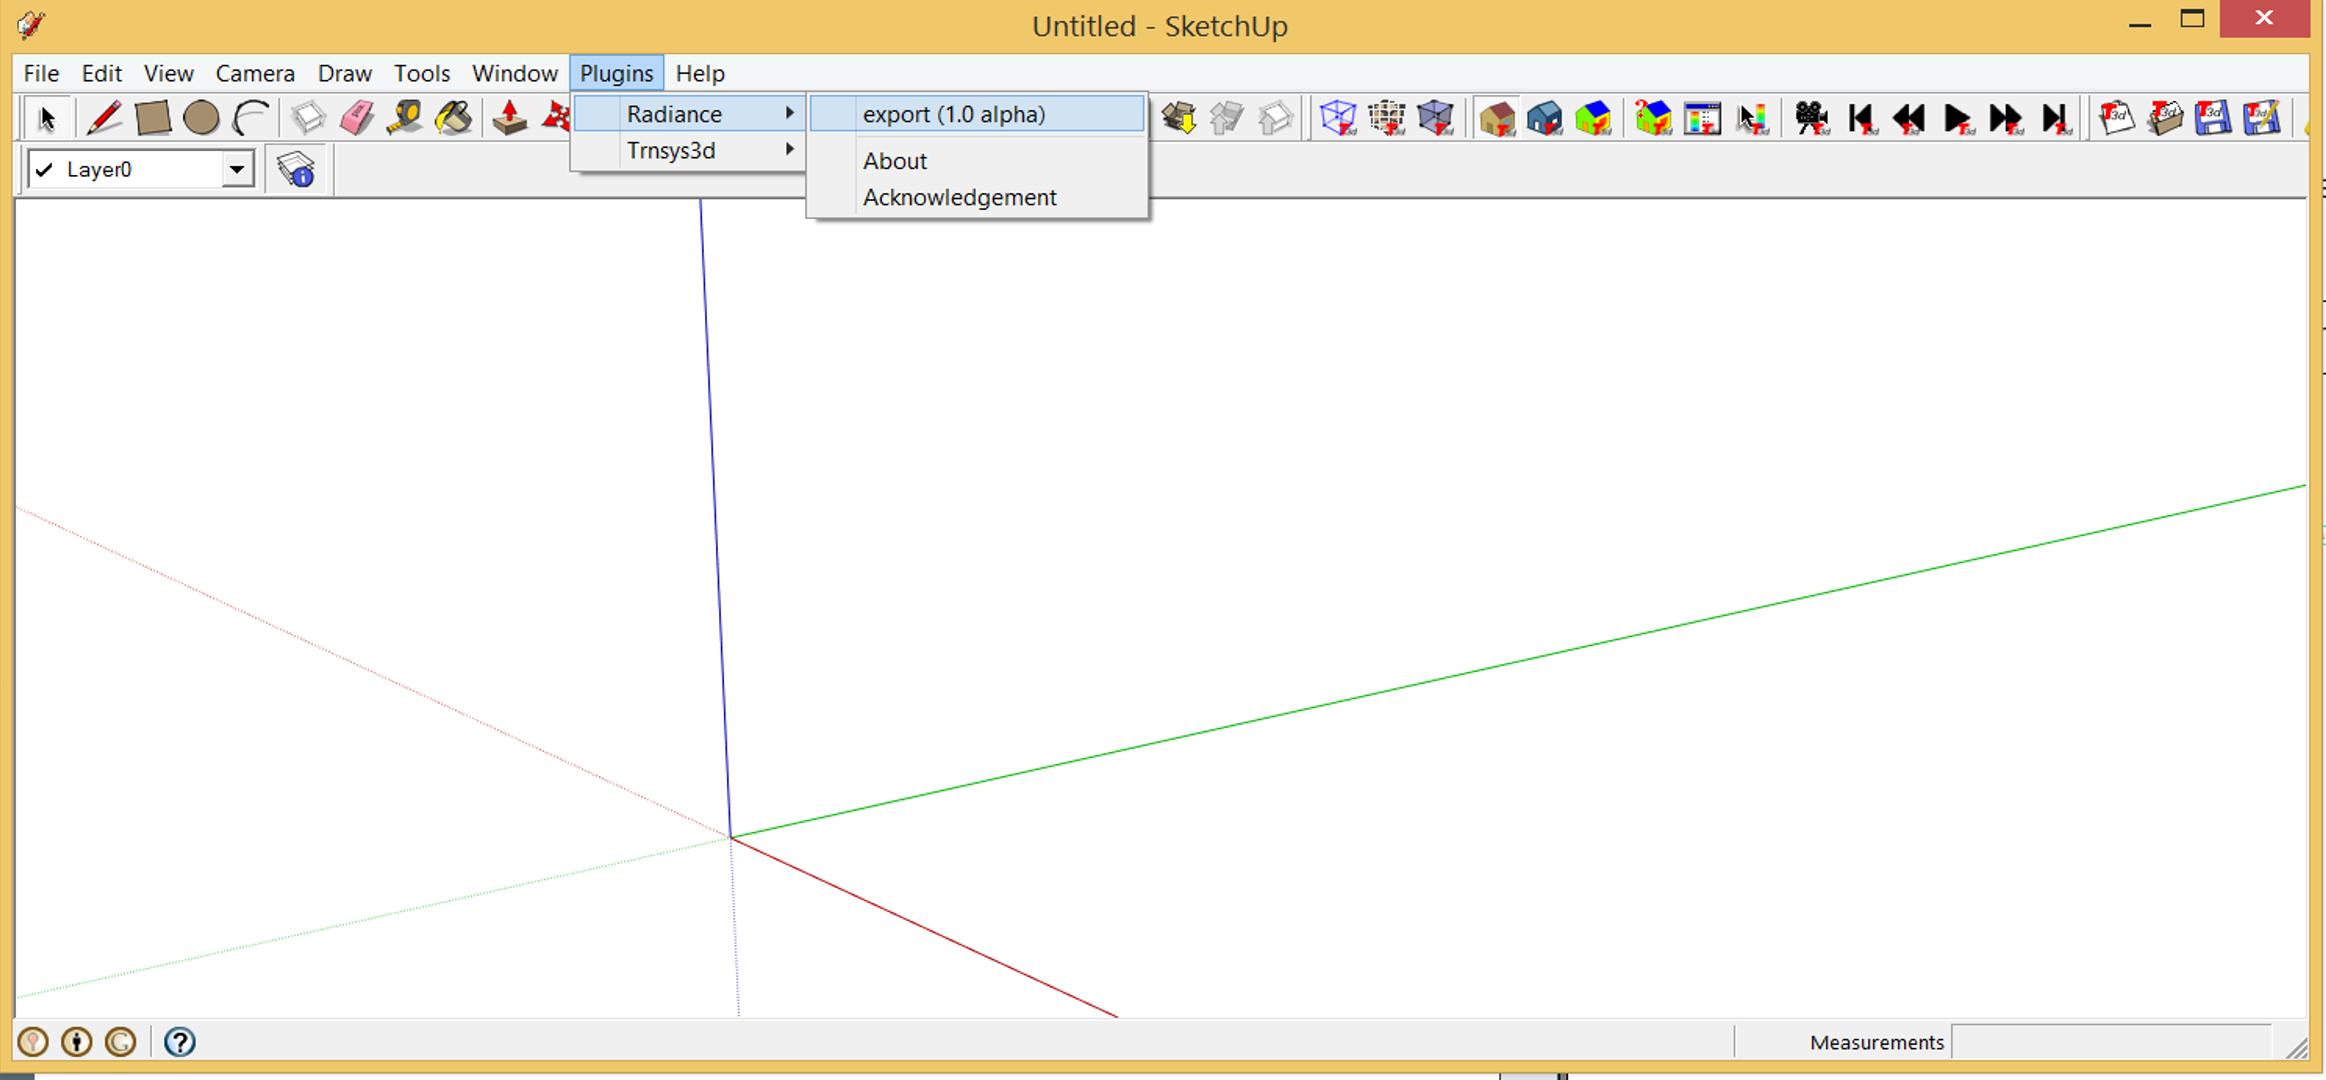
\includegraphics[width=0.9\textwidth]{su2rad}
\caption{\label{img1:su2rad} Initial screen in SketchUp with su2rad installed}
\end{figure}

\section{Draw a model}

Draw a model is very simple thanks to the user-friendly interface and the tools of SketchUp. As example we will create a shoe-box with an opening for the window on the south side of dimension 5x8x2.7 m. First, it is necessary to draw a horizontal surface that will be the plan of our box with the \textit{Rectangle} tool and then extrude this surface with the \textit{Push/Pull} tool, giving the third dimension to the box. The box will appear as the one in figure \ref{img1:box}. The orientation of the cardinal points as recognized by Radiance are also shown in the figure \ref{img1:su2rad}, the north-south direction is on the green axis  and east-west on the red axis. The blue axis points toward the sky.

\begin{figure}[h]
\centering
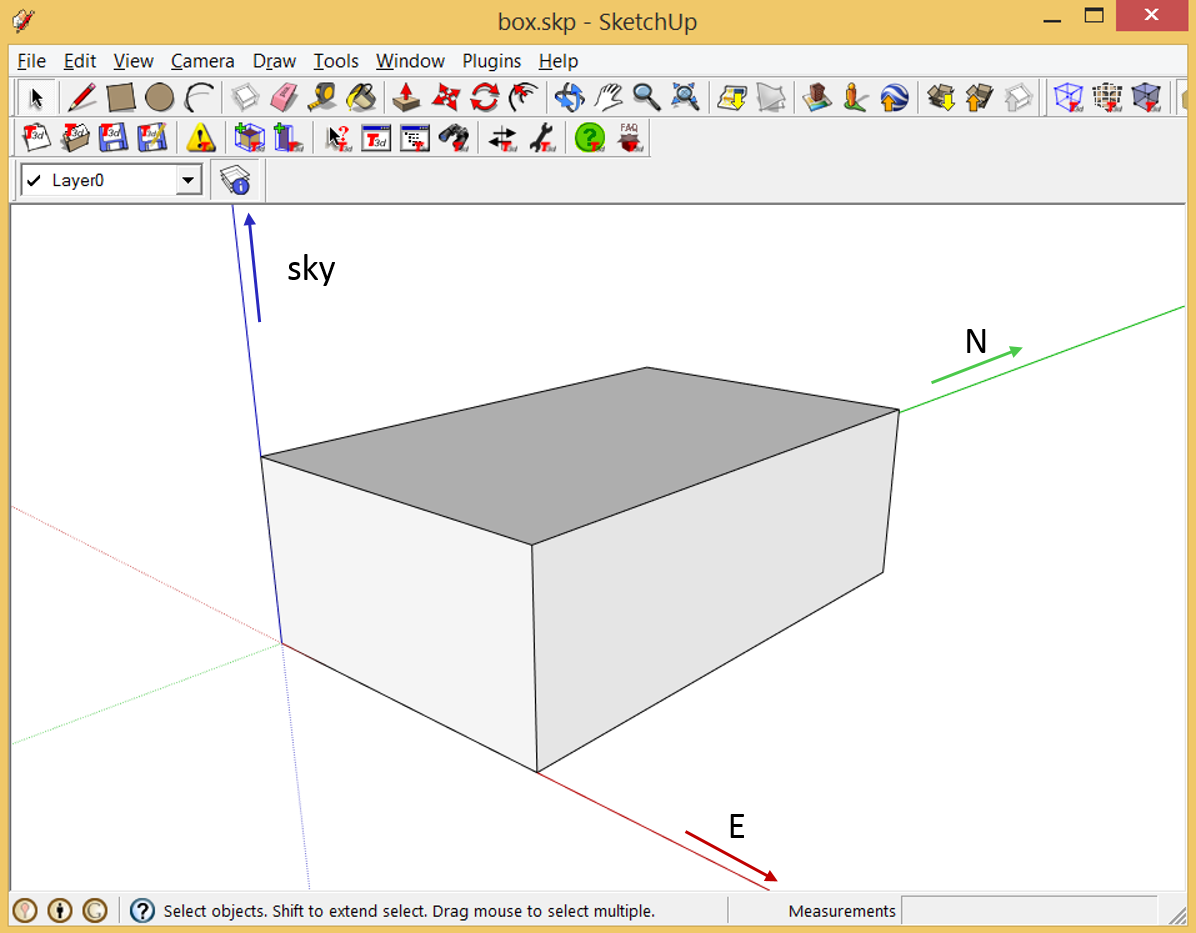
\includegraphics[width=0.9\textwidth]{box2}
\caption{\label{img1:box} Shoe-box drawn in SketchUp}
\end{figure}

Now it is necessary to draw the window on the south fa\c{c}ade. Select the \textit{Rectangle} tool and draw a rectangle on the vertical surface of dimension 3x1.2 m, distant 1 m from the side corner and 0.9 m from bottom. At this point assign a material to this new surface, open the \textit{Paint Bucket} and select a translucent glass material and click on the window surface. This step is not strictly required just because the material are set in a second phase, but it is useful to find easily the window in scene and have a overall idea of the geometry. Add also a ground surface to the scene, again using the \textit{Rectangle} tool. The box in figure \ref{img1:boxWin} is obtained. 

\begin{figure}[h]
\centering
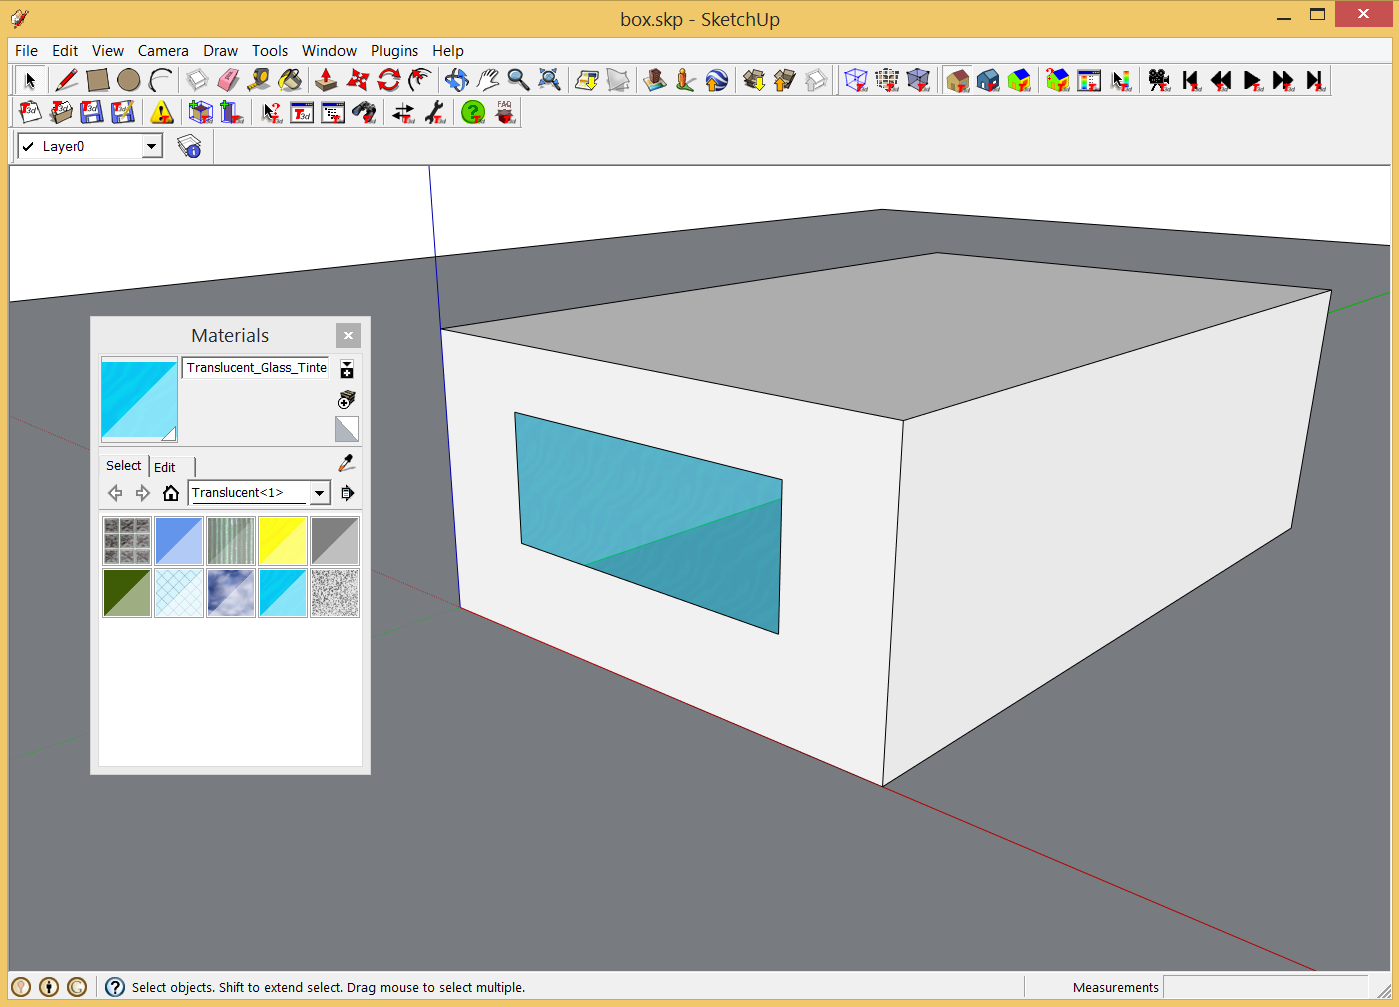
\includegraphics[width=0.9\textwidth]{boxWin2}
\caption{\label{img1:boxWin} Shoe-box with window on south fa\c{c}ade}
\end{figure}

Once the geometry is complete, the materials for each group of component has to be assigned. Assign at each layer a material and collect in each layer the surfaces with the same material/reflectance factor. This method allows to change very easily the material within Radiance. To do this open the layer window from \textit{Window -> Layers} and add as many layer as required by clicking on the "+" button. The common approach is set the layer as the main elements of the building that have the same reflectance: internal walls, 
external walls, ceiling, floor, Windows, ground, etc. Do not let space between the words in the name of the layer (i.e. layer Internal walls became Internal\_walls).

The procedure to move one or more surfaces from one layer to another is:
\begin{enumerate}
\item Select one or more surfaces. The selected entities are highlighted as dotted surfaces.
\item Activate the context menu for the selected entities, right click of the mouse.
\item Select the \textit{Entity Info} menu item. The Entity Info dialog box appears.
\item Select the layer for the entities from the 'Layers' drop-down list, figure \ref{img1:layer}.
\end{enumerate}

After moved all the surfaces in the respective layers, export the geometry created in a Radiance geometry. Before to export, place the view into the room and direct it toward the window (figure \ref{img1:inside}). This will be export in a Radiance view file that is useful to check if the window surface normal faces into the room (see section \ref{sec:normalsurf}). \\


\begin{figure}[h]
\centering
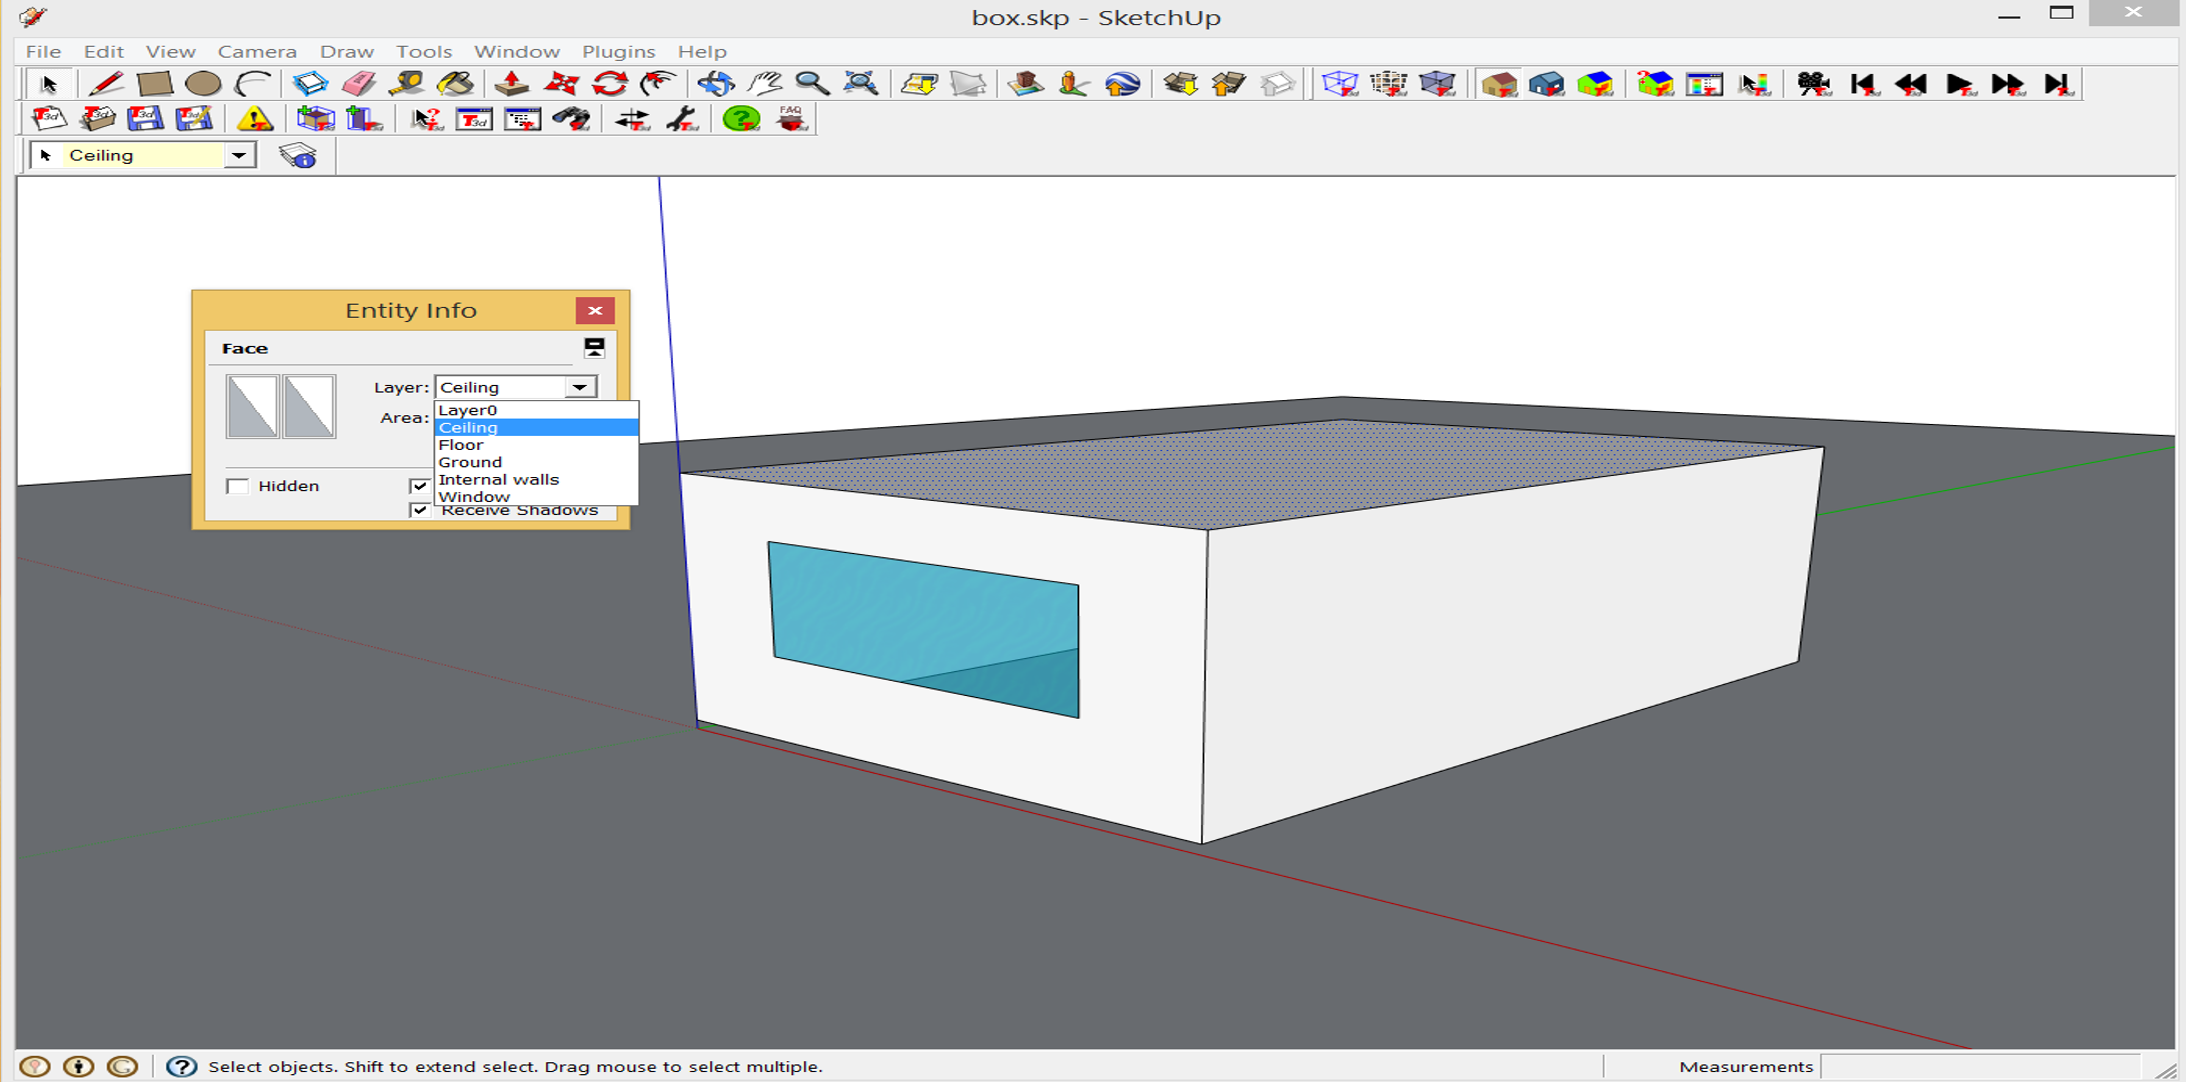
\includegraphics[width=0.9\textwidth]{layer}
\caption{\label{img1:layer} Definition of the surface in the respective layer}
\end{figure}


\begin{figure}[H]
\centering
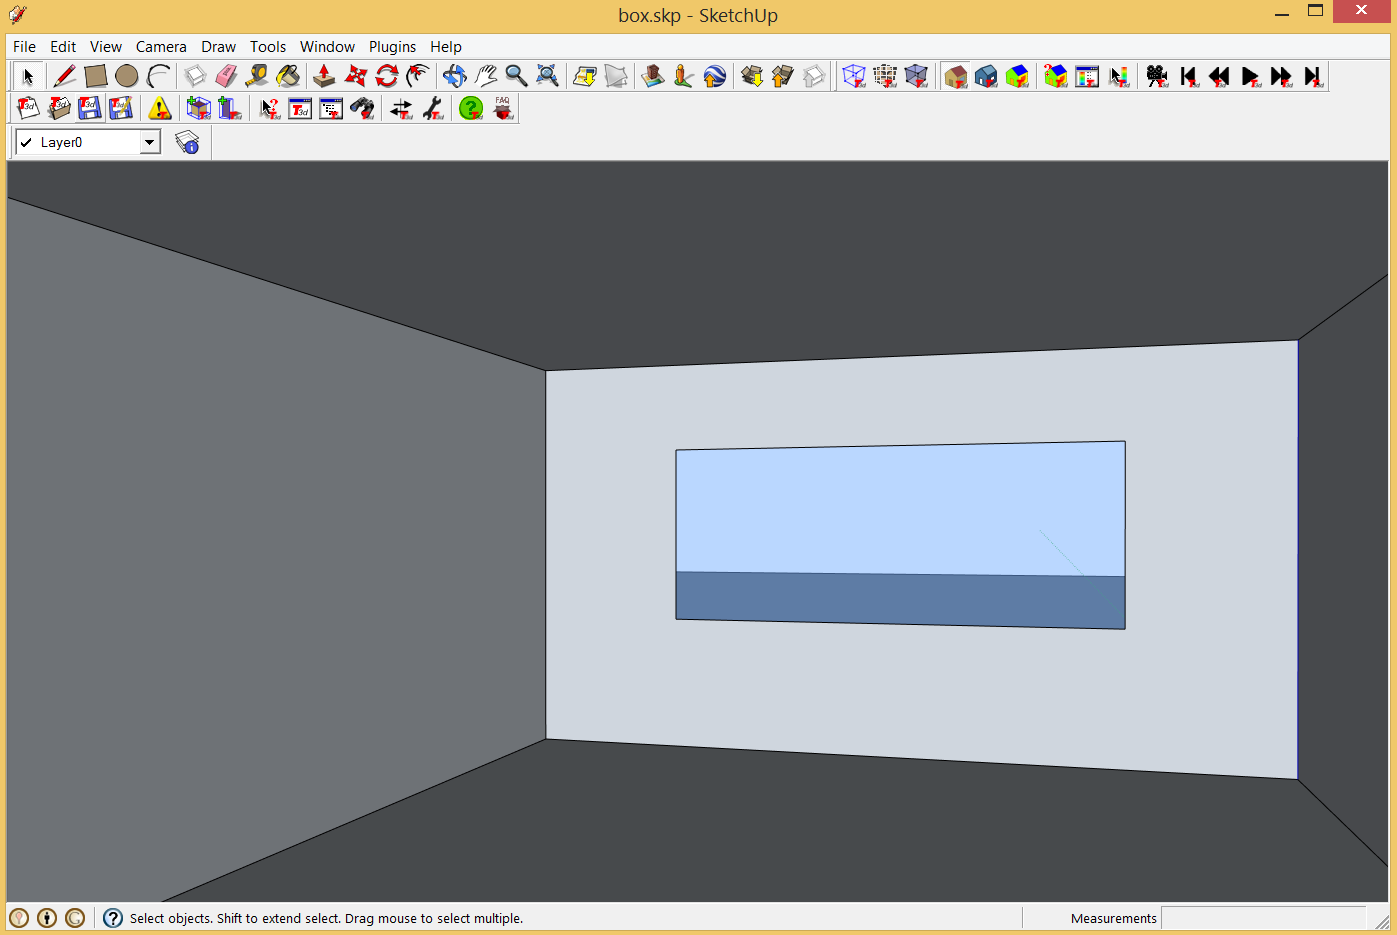
\includegraphics[width=0.9\textwidth]{insideview}
\caption{\label{img1:inside} View inside that will be used to check the direction of the window surface normal}
\end{figure}

\section{Export the model with su2rad} \label{sec:export}

Now export the Radiance geometry, open the su2rad export menu \textit{Plugins -> Radiance -> Export} (figure \ref{img1:export_menu}). Between the several windows available, you have to work on \textit{Export} (figure \ref{img1:export}), in which it is possible to define the path, the name of the scene and the mode. The name of the scene has to be defined considering the ID of the zone, that will be also the name of the folder containing the Radiance files (e.g. Zone1), see section \ref{sec:manualtweaks}. Regarding the exportation mode, case select "by layer" from the drop-down list. On the window \textit{Materials} (figure \ref{img1:materials}) the material for each layer can be set. \\
The SketchUp materials are displayed in three different ways:
\begin{itemize}
\renewcommand{\labelitemi}{\tiny$\blacksquare$}
\item Materials without corresponding names in the Radiance library are yellowish-brown. If there is no alias assigned to them for the export there will be a simple conversion of the SketchUp color.
\item Materials with corresponding names in the library are displayed in blue. They are exported with the definition from the library unless they are assigned another material.
\item Materials that have been assigned a Radiance definition are blue, too, and show the definition below the name. The definition from the library will be copied to the "materials.rad" file and an alias for the SketchUp material name will be added.
\end{itemize}
In order to assign a material to a SketchUp material/layer select the materials from the right column and drag it over the material/layer to the left. The color of the SketchUp material/layer will change to a darker shade and if you replace an existing material it will be outlined in red.
Below the two list of materials and layers, a window shows the definition of the Radiance material.

\begin{figure}[h] 
  \subfigure[Export menu]{% 
    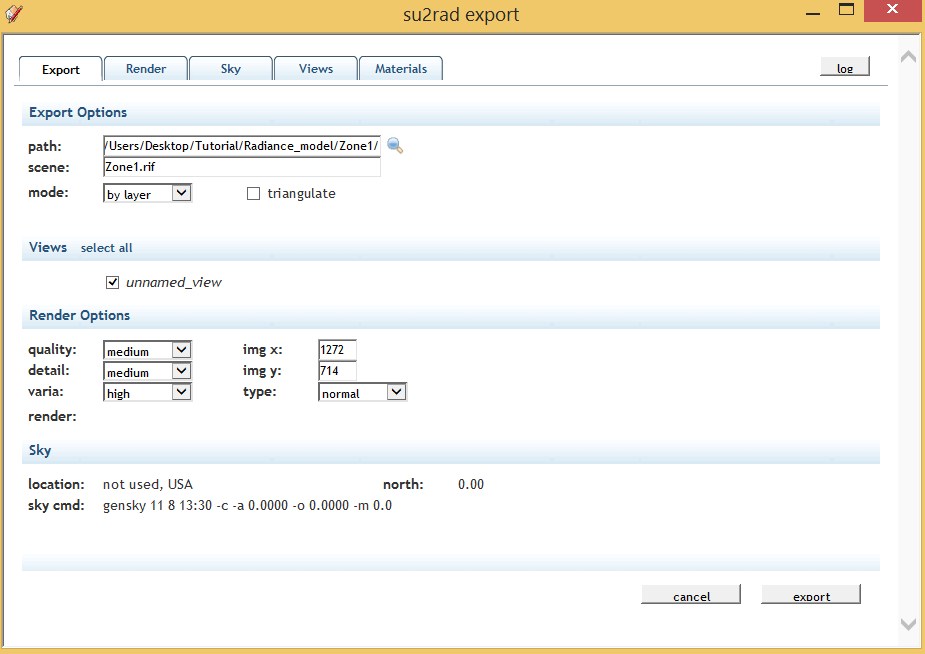
\includegraphics[width=.49\textwidth]{export2} \label{img1:export} 
  }
  \subfigure[Materials menu]{% 
    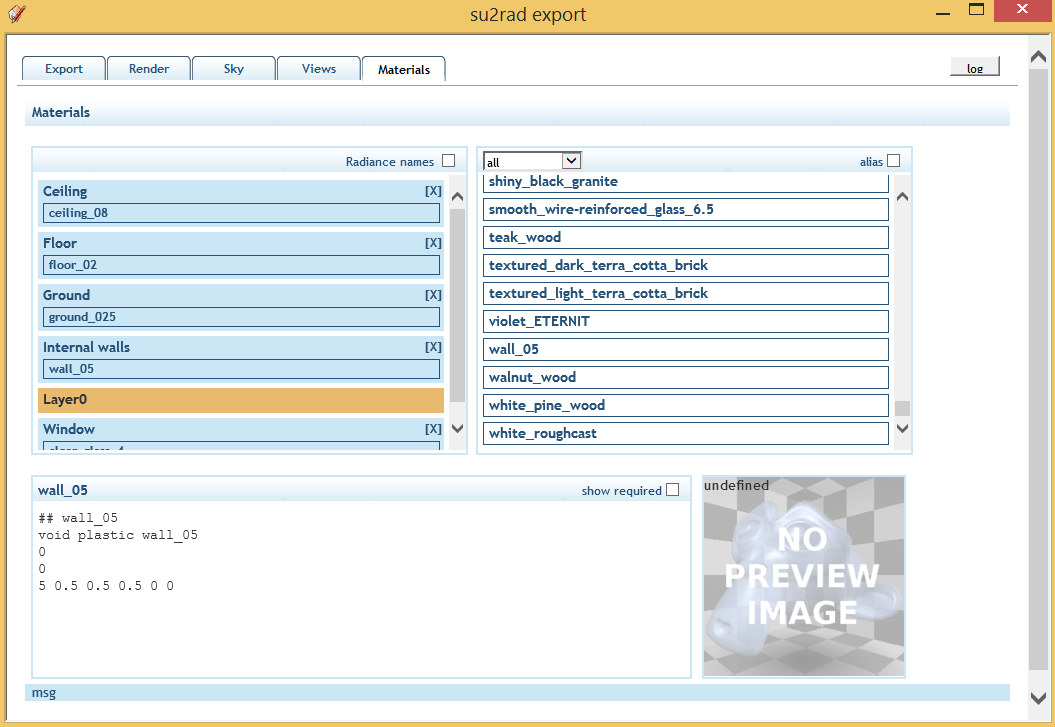
\includegraphics[width=.51\textwidth]{materials} \label{img1:materials} 
  } 
  \caption{\label{img1:export_menu} su2rad export options}
\end{figure}

Once all is set-up, export in Radiance geometry by clinking on export (figure \ref{img1:export}). In the path previously defined a new folder containing the new geometry will be created.

\begin{figure}[h]
\centering
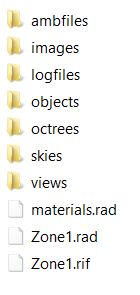
\includegraphics[width=0.2\textwidth]{exported}
\caption{\label{img1:exported} Contents of the folder export with su2rad}
\end{figure}


\subsection{Defining Custom Radiance Materials}
Probably, the default materials of su2rad are not useful for the user, therefore defining custom material became necessary. The ways to define custom materials are two:
\begin{enumerate}
\item adding the material to the su2rad library and assign it directly in SketchUp
\item creating the material manually and connecting it to the layer after the su2rad exportation
\end{enumerate}
First option allows also to reuse the material created for other models. 
In both cases the definition of the material has to respect the following syntax 
\begin{flalign*}
&<mod> <primitive> <id>\\
&<nargs> [args]\\
&<nargs> [args]\\
&<nargs> [args]\\
\end{flalign*}
The different definition of primitives and arguments depend of the material type, a deeper explanation and example of materials can be found in \url{http://radsite.lbl.gov/radiance/refer/ray.html#Materials} and \url{http://www.artifice.com/radiance/rad_materials.html}. \\
A useful tool for creating Radiance plastic and metal materials and seeing an high-quality preview of the material created is \textit{Radiance Colour Piker}, available at \url{http://www.jaloxa.eu/resources/radiance/colour_picker.shtml} by clicking on the button \textit{Launch the Colour Picker}. Once the material is generated, it can be copy and paste in the materials definition of Radiance scene.
\paragraph{Adding material in the su2rad material library}
Adding a material to the su2rad library is quite simple. First, move in the su2rad plungins folder and open the folder \textit{ray}, usually the path where find the folder is \textit{C:\textbackslash Program Files (x86)\textbackslash Google\textbackslash Google SketchUp 8\textbackslash Plugins\textbackslash su2radlib\textbackslash ray}.\\
Within the ray folder are present three file:
\begin{itemize}
\renewcommand{\labelitemi}{\tiny$\blacksquare$}
\item K\_and\_E.rad
\item  ral.rad
\item materials.rad
\end{itemize}
where ral.rad and K\_and\_E.rad contain materials corresponding to specific colour scales. Materials.rad contains more realistic material (e.g. wood, concrete, etc.). The latter file is the one that has to be modified. Before modifying the file, create a backup copy of it and rename as \textit{materials\_orginal.rad}.\\
Open the material.rad with notepad (or equivalent software) and add at the bottom of the file the material just created. In figure \ref{img1:materialrad} has been also created a section within the file called "My materials" useful to identify immediately where the custom materials are located.
\begin{figure}[h]
\centering
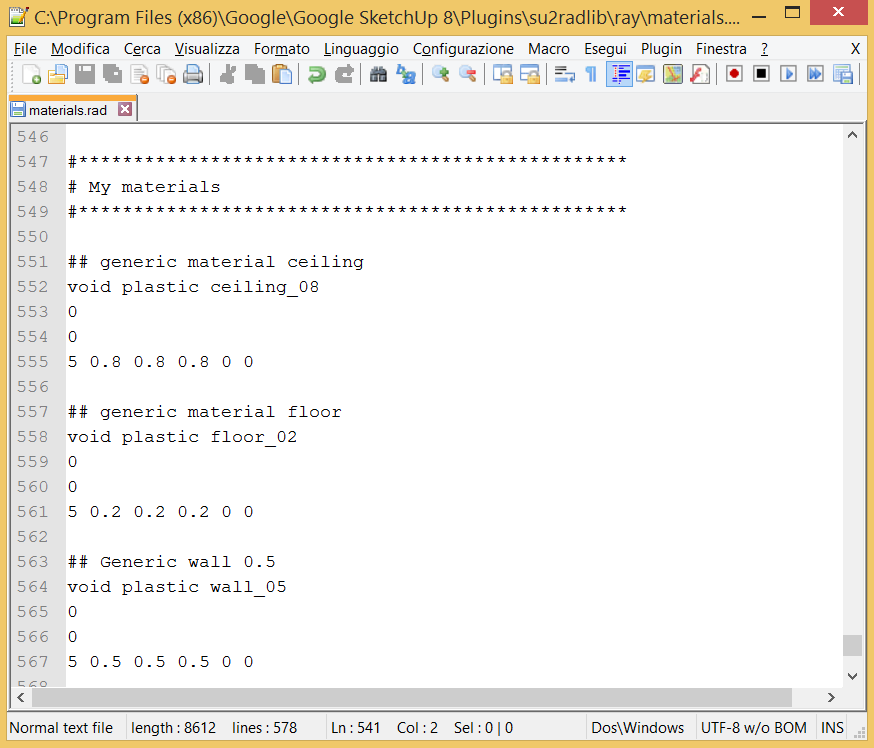
\includegraphics[width=0.7\textwidth]{materialrad}
\caption{\label{img1:materialrad} Definition of custom materials within the su2rad material library}
\end{figure}
Once a material has been added to the library, it became available in SketchUp and can be associate to a layer in the material window in figure \ref{img1:materials}.

\paragraph{Adding material in the material.rad file exported}
If no material is assigned in SketchUp, then SketchUp will assign a default material to each layer. The material.rad file exported by su2rad will appear as in figure \ref{img1:materialexported}. Delete the SketchUp default material and write your materials keeping in mind two important things:
\begin{itemize}
\renewcommand{\labelitemi}{\tiny$\blacksquare$}
\item use the syntax shown at the begin of this section
\item use for the ID of the material the name of the MODIFIER of the object (in this case the name of the layer, e.g. ceiling, floor, etc.) to combine material and geometry, as shown in figure \ref{img1:combine}
\end{itemize} 
Once created the material for each layer and wrote them in to the materials.rad file it will seem like in Figure \ref{img1:materialmodif}.
\begin{figure}[h]
\centering
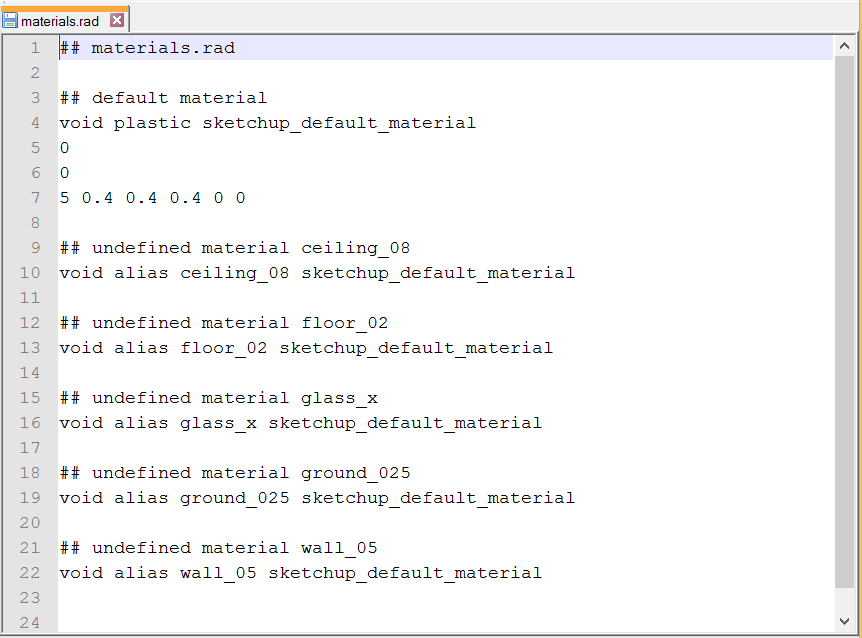
\includegraphics[width=0.7\textwidth]{materialexported}
\caption{\label{img1:materialexported} material.rad exported with default SkectchUp materials}
\end{figure}


\begin{figure}[h]
\centering
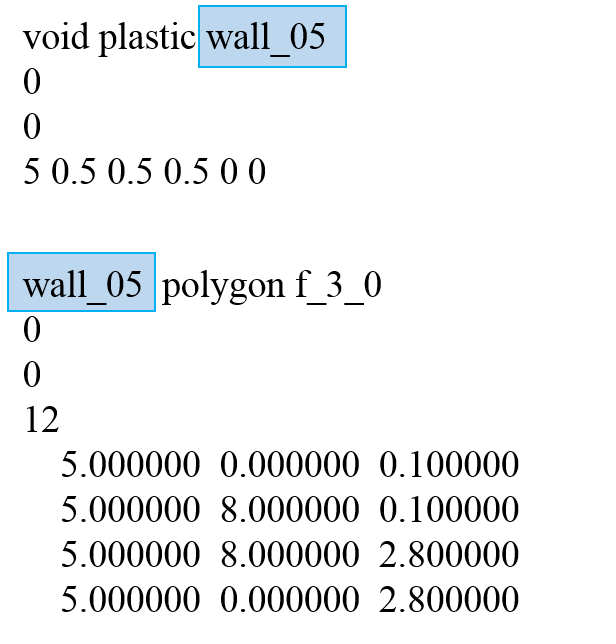
\includegraphics[width=0.4\textwidth]{combine}
\caption{\label{img1:combine} Combine the material and the geometry using the MODIFIER of the object as ID of the material}
\end{figure}

\begin{figure}[h]
\centering
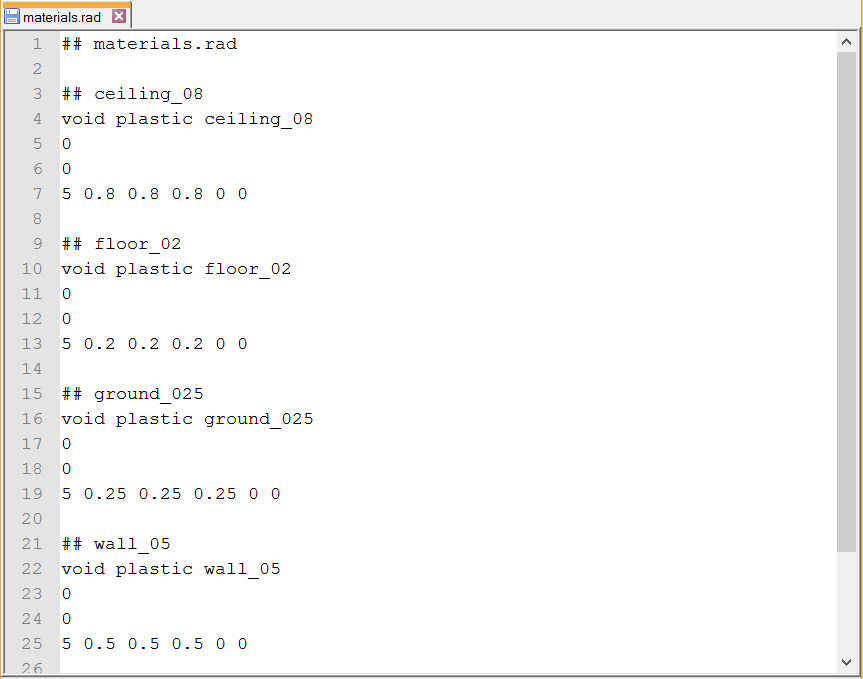
\includegraphics[width=0.7\textwidth]{materialmodif}
\caption{\label{img1:materialmodif} materials.rad with the materials defined by the user}
\end{figure}



